\chapter{Haptic Design}
This chapter briefly touches on the field of haptics and delves into tactile research. This leads into a discussion of the overall design requirements, initial prototypes, and overall challenges overcome which led to the development of the final prototype, the vibrotactile array.

\section{Brief introduction to haptics}
\textbf{Haptics} are the field of research which concern the sense of touch as it applies to \textit{kinesthetic} and \textit{tactile} sensation. The tactile sense enables humans to perceive object properties through skin contact while the \textit{kinesthetic} or \textit{proprioceptive} sense lets one perceive the positions, movements, and forces on one's own body. 

The skin is lined with an array of sensory receptors which respond to mechanical pressure and distortions such as skin deformation. The \textit{lamellated} or \textit{pacinian corpuscles} (PC) are responsible for sensitivity to vibration and pressure. These rapidly adapting receptors are responsible for vibrotactile perception in glabrous skin. 

Sensitivity to a tactile stimulus grows with the area in contact with the skin and also improves with the stimulus duration until it is saturated. When pressure is continuous an effect called \textit{haptic masking} or the \textit{summation effect} is possible. The \textit{pacinian corpuscles} become saturated with the concentrated stimulus such that the brain ignores these messages with a mechanical filtering system which lowers the perception threshold in order to focus on other important happenings. If this was not the case, a person could for example feel the pressure exerted by wearing clothing \cite{choi2013vibrotactile}. This phenomena is important to consider when dealing with haptic placement. As mentioned in \ref{tactileModality}, when the vibrotactiles were placed over a larger area span the results closely matched the auditory modality.

\subsection{Haptic Considerations}
The following questions arise based on extensive research done by Choi and Kuchenbecker \cite{choi2013vibrotactile} and are crucial concepts underpinning the creation a meaningful haptic.
\begin{enumerate}
    \item \emph{Can the user feel it?}
Vibrotactile stimuli perceptibility is strongly dependent on the frequency of vibration. The minimum threshold is observed to be between 150-300Hz and can cover an area smaller than 0.1 micrometer. The absolute thresholds are dependent on factors such as body site, contact area, stimulus duration, stimulus waveform, contact force, skin temperature, presence of other masking stimuli, and age.

    \item \emph{Can the user distinguish between the different vibrotactile cues being displayed?}
This is quantified by the discrimination or \textit{difference threshold} also called the \textit{Just Noticeable Difference} (JND). It is defined as the smallest amount a stimulus intensity much change to produce a noteable change in sensory experience. The JND is measured as a \textit{Weber fraction}:
${\Delta}$I/I = k or the ratio of difference threshold to the reference level.
Research into experimental psychology has deemed a 20-30\% difference in amplitude or frequency is necessary for robust discrimination between vibrotactile stimuli in practical applications.

    \item \emph{How strong does a certain vibrotactile cue feel to the user?}
\textit{Steven's power law} describes the relationship between the magnitude of a physical stimulus and its perceived intensity or strength. See Figure \ref{fig:StevensPowerLaw}
\begin{figure}[H]
    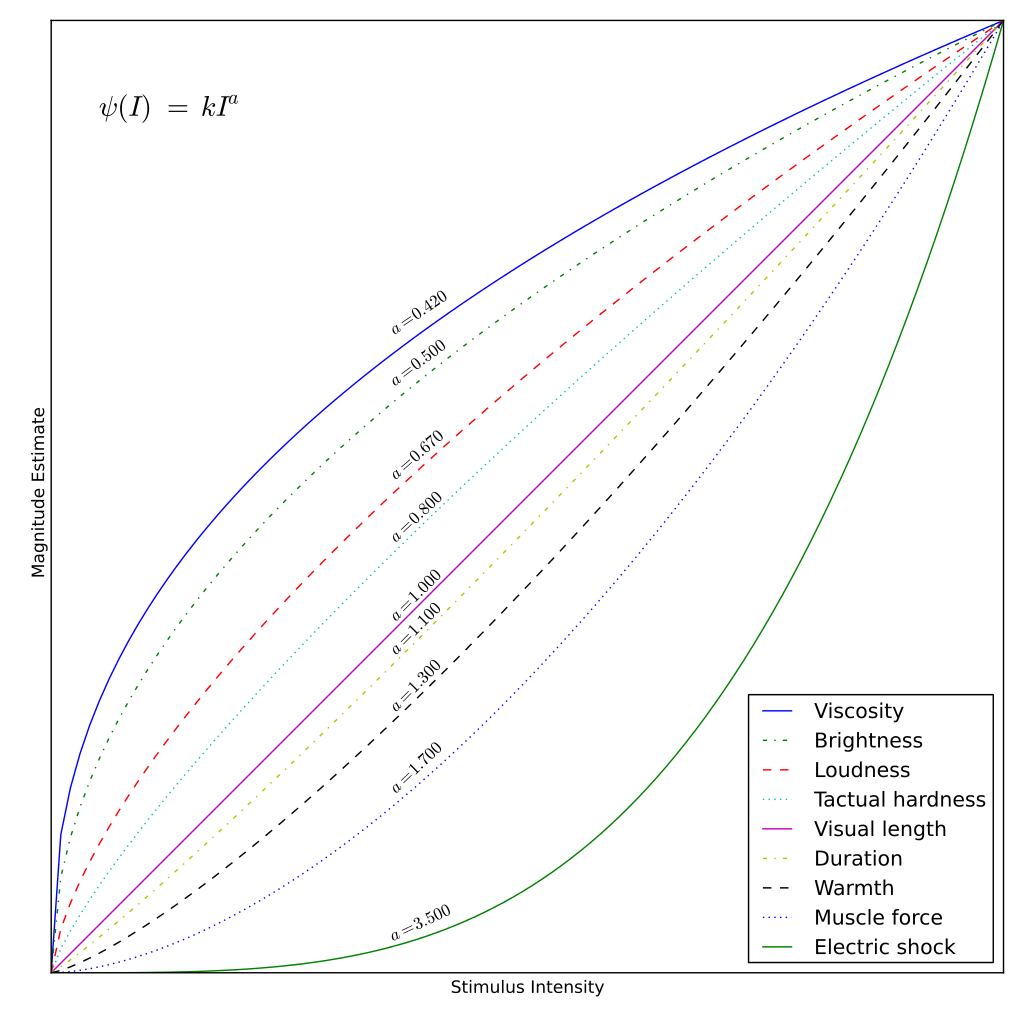
\includegraphics[width=\linewidth,height=\textheight,keepaspectratio]{Steven's_Power_Law}
    \label{fig:StevensPowerLaw}
\end{figure}
    \begin{itemize}
        \item when a stimulus intensity \textit{I} is above its absolute threshold, humans perceives its magnitude as \begin{math}\Psi(I)\end{math}(perceptual strength)
        \item the exponent (dependent on stimulation freq) determines growth rate of the perceived magnitude, ranges from 0.35 to 0.86 for vibrotactiles
        \item perceived intensity is a function of freq and amplitude of vibration (also affecting perceived pitch)
    \end{itemize}
    \item \emph{How good are users at judging timing of vibrotactile cues?}
    \begin{itemize}
        \item tactile perception is generally considered to have high temporal acuity
        \item vibrotactile temporal resolution research cites a humans ability to distinguish successive pulses with a time gap as small as 5 ms (12000 BPM)
        \begin{itemize}
            \item this resolution is better than vision (25ms) but slightly worse than physiological experiments into the peripheral auditory system which cites a theoretical best case scenario of approximately 2 ms \cite{fishbach2001auditory} \cite{parsons2006neurobiology}
        \end{itemize}
    \end{itemize}
    \item \emph{Can Vibrotactile cues elicit any other perceptual effects?}
    \begin{itemize}
        \item below 3 Hz considered slow kinesthetic motion
        \item between 10-70Hz is the sensation of rough motion or fluttering
        \item between 100-300Hz is the sensation of smooth vibration
        \item subjective quality of a vibrotactile stimulus can be controlled by modifying the envelope of the stimulus amplitude
    \end{itemize}
\end{enumerate}

\subsection{Vibrotactiles}
The exploration of touch actuation led to the evaluation of available vibrotactiles. The following is a thorough breakdown to inform design perspective.
\begin{enumerate}
    \item Linear electromagetic actuators
    \begin{itemize}
        \item solenoid:
        \begin{itemize}
            \item can leverage resonance, large output for small input
            \item force dependent on position within magnetic field
            \item influenced by device orientation relative to gravity
            \item heats up during use
        \end{itemize}
        \item voice coil:
        \begin{itemize}
            \item linear dynamics yields consistent output, relatively easy to model
            \item \textit{C2 tactor}:
            \begin{itemize}
                \item 7.6mm contactor preloaded against the skin
                \item suspension resonates at 250Hz for maximum perceptibility
            \end{itemize}
            \item \textit{Haptuator}:
            \begin{itemize}
                \item moving magnet design
                \item not meant to touch the skin
                \item optimized to render frequencies above 50Hz
            \end{itemize}
        \end{itemize}
    \end{itemize}
    \item Rotary Electromagnetic Actuators (ERM - eccentric rotating mass)
    \begin{itemize}
        \item simple, reliable, rotate continuously with a constant voltage/current applied
        \item off-center mass affixed to output shaft so that its rotation exerts large radial forces on the body of the motor
        \item couples freq and amplitude of the resulting vibration to the motors rotational speed
        \item small voltage yields weaker vibrations
        \item intrinsic spin-up time could cause delay at the start of the cue
        \item internal static friction can prevent motor from rotating when the applied voltage is very small
    \end{itemize}
    \item Nonelectromagnetic Actuators - Piezoelectric effect
    \begin{itemize}
        \item respond to inputs very quickly and can output arbitrary waveforms
        \item typically require input on the order of 100V
        \item high stiffness of skin creates a need for relatively heavy vibrotactile actuator
        \item most don't have power to move the skin without pushing off a cumbersome mechanical ground
    \end{itemize}
    \item EAP (electroactive polymer) actuators
    \begin{itemize}
        \item uses elastomers rather than ceramics
        \item can achieve larger deformations for lower drive voltages
    \end{itemize}
    \item SMA (shape memory allow) actuators
    \begin{itemize}
        \item remembers original shape
        \item mechanical properties altered in response to temp changes
        \item slow response time, large hystoresis, high energy consumption
    \end{itemize}
    \item Pneumatic systems
    \begin{itemize}
        \item compact, light
        \item require high-pressure air source
        \item struggle to output high-frequency signals
    \end{itemize}
    \item Forced impact
    \begin{itemize}
        \item TacHammer - new technology, specs unknown, hard to acquire
    \end{itemize}
\end{enumerate}

\subsubsection{Vibrotactile Constraints}
-create consistent mechanical coupling between actuator vibrations and users skin
-slight changes to such a system drastically affect users ability to feel and comprehend the rendered signals.
-for fixed actuator size/activation level, magnitude of created vibrations is inversely proportional to the mass of the object (minimize overall weight of device)
-small high-BW accelerometer to measure vibration output performance
-when the application involves a large object, a wearable device, and/or multiple stimulation sites, the optimal vibrotactile rendering paradigm is to vibrate one or more small zones.

For example, the localization accuracy of 250-Hz vibrotactile stimuli around the waist was 74\% with 12 equidistant tactile actuators (tactors), 92\% with eight tactors, and 97\% with six tactors 		



\section{Design requirements}

The initial requirement set forth by Professor Neely in the Haptic Enviro-Sensing Metronome (HESM) design draft is centered around an analogue wave that could squeeze and release. As the analogue wave approaches its crest it provides insight forecasting the approaching \textit{crusis}, allowing the user to prepare for and rebound from the "click-moment" with rich entrainment. 

This observation is in direct parallel to external vibrotactile metronome research as discussed in \ref{vibrotactileMetronome}. The constraint was such that the pulses should feel continuous and not discrete, even mentioning a pendulum motion as the descriptive feeling to convey. 

As the intention is to encourage entrainment of the human body to external forces, the frequencies
required are quite low, based on the tempi of slow walking to running gaits
(40 bpm/.67 Hz to 180 bpm/3 Hz).

\cite{Neely}
\todo[inline]{add HESM design to bio for citations}

\section{Initial Prototypes}
In order ot capture the sensation defined in the design requirements, a series of prototypes were rapidly developed.

\subsection{Solenoid bracelet}
Initial introspection towards capturing this squeeze and release sensation led to the rapid prototyping of a simple solenoid bracelet. 

\subsubsection{Single vibrotactile}

\section{Vibrotactile Haptic Array}

\subsection{Hardware}


\subsection{Software}

\section{Design Challenges}

Motor noise

Managing power dips



Debounce for tap tempo

\section{Optimization}

\subsection{Future Implementation}

Bluetooth/Wireless

Custom PCB

Experiment with other vibrotactiles such as tachammer and LNA's
